
\section{}

% OK
\subsection{Exercise 0 (Simple attacks)}

Let $\MAC = (\Gen, \Mac, \Vrfy)$ be existentially unforgeable under an adaptive chosen-message attack and let $\Pi=(\Gen, \Enc, \Dec)$ be a CCA-secure scheme. Consider the following schemes $\MAC'=(\Gen', \Mac', \Vrfy')$ (resp. $\Pi'=(\Gen', \Enc', \Dec')$) based on $\Mac$ with $\Gen'=\Gen$ and $\Mac'$ (resp. $\Gen=\Gen'$ and $\Enc'$) defined as follow:
\begin{enumerate}
	\item $\Mac'_k(m) \define (\Mac_k(m), \Mac_k(m\xor 0\dots01))$
	\item $\Mac'_k(m) \define \Mac_k\left(\bigoplus_{i=1}^l m_i \right)$
	\item $\Mac'_k(m) \define (\Mac_k(m_1), \dots, \Mac_k(m_l))$
	\item $\Mac'_k(m) \define (\Mac_k(m_1), \Mac_k(m_1||m_2), \dots, \Mac_k(m_1||\dots||m_l))$
	\item $\Enc'_k(m) \define \left(\Enc_k(m), \Enc_k\left(\bigoplus_{i=1}^l m_i\right)\right)$
	\item $\Enc'_k(m) \define \left(\Enc_k(m), \bigoplus_{i=1}^l m_i\right) $
	\item $\Enc'_k(m) \define (\Enc_k(m), \Enc_k(m \oplus 110\dots0))$
	\item $\Enc'_k(m) \define (\Enc_k(m||0), \Enc_k(m))$
\end{enumerate}
Break all $\MAC'$ and $\Pi'$.

(In some cases $m$ is parsed in $m_1,\dots,m_l$ with $|m_1|=\dots=|m_{l-1}|=n$, $|m_l| \le n$ and $m_1||\dots||m_l=m$ ($||$ is the concatenation) where $n$ is the security parameter.)


\begin{solution}
	The following are sketches of the attacks that need to be performed; a correct answer needs to define the setting of the attack, in a manner similar to the reduction proofs.
	\begin{enumerate}
		\item Let's build an adversary $\A$ that can break the $\MAC'$ scheme. Let's define the following experiment $\MacForge_{\A,\Pi'}(n)$ (in the viewpoint of the adversary):
		\begin{enumerate}[label=(\arabic*)]
			\item The oracle-challenger chooses $k \pick \K$.
			\item We are given access to an oracle for $\Mac'_k(\cdot)$; this oracle records all requested messages in $Q$. With $m \define 0\dots0$, we ask for $t \define \Mac'_k(m)$ and receive $t=(t_1, t_2)$ with $t_1=\Mac_k(m)$ and $t_2=\Mac_k(m \oplus 0\dots01))$.
			\item We output $m^*=0\dots01$ and $t^*=(t_2, t_1)$.
			\item Define $\MacForge_{\A,\Pi'} \define 1$ iff $\Vrfy'_k(m^*, t^*) = 1$.
		\end{enumerate}
	Observe that
	\begin{align*}
	\Mac'_k(m^*) &= (\Mac_k(m^*), \Mac_k(m^* \oplus 0\dots01)) = (\Mac_k(0\dots01), \Mac_k(0\dots01 \oplus 0\dots01)) \\
	&= (\Mac_k(0\dots01), \Mac_k(0\dots0)) = (t_2, t_1)
	\end{align*}
	and so, the pair $(m^*, t^*)$ is indeed a valid tag. In addition, the message $m^*$ is different from $m$ and so $m^*\not\in Q$.
	Thus, $\Pr[\MacForge_{\A,\Pi'}=1] = 1$ which is clearly not negligible.

	\item We ask $m=0\dots0||0\dots01$ to the oracle as a message consisting of two blocks of length $l$, and receive the tag $t=\Mac'_k(m)=\Mac_k(0\dots0 \oplus 0\dots01) = \Mac_k(0\dots01)$.

	Then, we output $m^* \define 0\dots01||0\dots0$ and $t^* \define t$. Observe that $\Mac'_k(m^*)=\Mac_k(0\dots01 \oplus 0\dots0)=\Mac_k(0\dots01)=t=t^*$ and thus is a valid tag for a message not asked to the oracle.

	\item We send to the oracle $m=0\dots0||0\dots01$ as a two-blocks message and receive $t=\Mac'_k(m)=(\Mac_k(0\dots0), \Mac_k(0\dots01))=(t_1, t_2)$. We output $m^*=0\dots01||0\dots0$ and $t^*=(t_2, t_1)$. Observe that $\Mac'_k(m^*)=(\Mac_k(0\dots01), \Mac_k(0\dots0))=(t_2, t_1)=t^*$, and $m^*$ was not asked to the oracle, so this is a valid pair.

	\item We send $m=m_1||m_2$ for some message blocks $m_1, m_2 \pick \bset^n$ (they don't matter) and receive $t=\Mac'_k(m)=(\Mac_k(m_1), \Mac_k(m_1||m_2))=(t_1, t_2)$. We output $m^*=m_1$ and $t^*=(t_1)$. Note that this requires $\Mac_k(\cdot)$ and $\Mac'_k(\cdot)$ to accept arbitrary-length messages, and $\Mac'_k(\cdot)$ to output arbitrary-length tags.

	\item We ask the oracle to encrypt $m=0\dots01 || 0\dots01$, a two-blocks message and receive $c=(c_1, c_2)=(\Enc_k(m), \Enc_k(0\dots01 \oplus 0\dots01))=(\Enc_k(m), \Enc_k(0\dots0))$.
	We then output $m_0=0\dots0||0\dots0$ and $m_1=1\dots1||1\dots1$.
	Observe that $\bigoplus_{i=1}^l m_{0,i} = \bigoplus_{i=1}^l m_{1,i} = \bigoplus_{i=1}^l m_{i}=0\dots0$.
	We receive $c=(c^*_1, c^*_2)=(\Enc_k(m_b), \Enc_k(\bigoplus_{i=1}^l m_{b,i}))=(\Enc_k(m_b), \Enc_k(00\dots00))$.
	We then ask to decrypt $c^*=(c^*_1, c_2)$ and will receive $m_b$.

	This assumes that the two encryptions that take place in $\Enc'$ are independent (e.g., use different $r$) so that we can combine the two parts in arbitrary ways.
	Also, there is a slight chance that $c_2=c^*_2$ (if both encryptions used the same random values) as they encrypt the same message. If $n$ is the number of bits of the random values used in the encryption (e.g., the number of bits of $r$), then this probability is $\frac{1}{2^n}$ which is negligible.

	\item We output $m_0=0\dots0$ and $m_1=0\dots01$ with length $n$ (so that the messages are not split). Then, receiving $c=(\Enc_k(m_b), \bigoplus_{i=1}{l}m_b)=(\Enc_k(m_b), m_b)$, we answer $0$ if $m_b=m_0$ and $1$ otherwise.

	\item We output $m_0=0\dots0$ and $m_1=1\dots1$, and receive $c=(\Enc_k(m_b), \Enc_k(m_b\oplus 110\dots0))=(c_1, c_2)$. We then ask the oracle to decrypt $c^*=(c_2, c_1)$ (this is not $c$) and receive $m^*=m_b\oplus 110\dots0$. We then just have to compute $m'=m^*\oplus 110\dots0$ and compare with $m_0$ and $m_1$ to identify it. For this attack to work, we need a decryption oracle, and so need to play the CCA security game.

	\item We output $m_0=0\dots0$ and $m_1=1\dots1$ and receive $c=(\Enc_k(m_b||0), \Enc_k(m_b))=(c_1, c_2)$. We ask the oracle to decrypt $c^*=(c_2, c_1)$ and should receive $m_b||0$ or $m_b$.

	Note: this attack looks wrong, as it requires $\Dec'$ to ignore the fact that, in theory, the first part of the ciphertext encrypts the same message as the second part, with a $0$ appended. In practice, decrypting such malformed messages should result in an error. But it was the ``official'' answer.
	\end{enumerate}
\end{solution}



% OK
\subsection{Exercise 1 (Fixed-length MAC)}

Consider the fixed-length MAC $\Pi \define \langle\Gen,\Mac,\Vrfy\rangle$
defined as follows:
\begin{itemize}
  \item $\Gen$: choose random $k\leftarrow \bset^n$
  \item $\Mac$: on input $m,k \in\bset^n$, output $t \define F_k(m)$
  \item $\Vrfy$: on input $k, m, t \in \bset^n$ output 1 iff $t=F_k(m)$
\end{itemize}

Prove that, if $F$ is a PRF, $\Pi$ is existentially unforgeable under
an adaptive chosen-message attack. Hint:

\begin{enumerate}
  \item Consider the scheme $\Pi'$ defined as $\Pi$ except that a truly
        random function is used instead of a pseudo-random one. Show that
        $\Pi'$ is existentially unforgeable under an adaptive chosen-message
        attack.
  \item Consider a PPT adversary who can produce an adaptive forgery on
        $\Pi$ with non negligible probability $\negl(n)$. Using this
        adversary, show that $F$ cannot be a PRF.
\end{enumerate}


% homework 2 of Dan Boneh, Winter 2011, Problem 2
\begin{solution}
  \begin{itemize}
    \item
      Let $\tilde{\Pi} = \langle \tilde{\Gen}, \tilde{\Mac}, \tilde{\Vrfy} \rangle$, defined as:
      \begin{itemize}
        \item $\tilde{\Gen}$: chooses a random $f$.
        \item $\tilde{\Mac}$: on input $m$, outputs $f(m)$.
        \item $\tilde{\Vrfy}$: on input $(m,t)$, outputs $1$ iff $f(m) = t$.
      \end{itemize}

      Let's analyse the maximum value of $\Pr[\MacForge_{\A, \tilde{\Pi}}(n) = 1]$ for an adversary $\A$.
      If after $q$ different queries (it gains no info doing the same query twice),
      $m_1, \dots, m_q$, $\A$ outputs $(m, t)$, what are its chances of success ?
      Let $f \colon \bset^n \mapsto \bset^n$.
      There are $(2^n)^{2^n}$ different $f$ and we pick a random one uniformly.
      However, there are only $(2^n)^{2^n-q}$ experiments such that $\A$ could have received $(m_i,t_i)$ for $i = 1, \ldots, q$ because
      there are $(2^n)^{2^n-q}$ $f$ such that $f(m_i) = t_i$ for $i = 1, \ldots, q$.
      We could be in any of them.
      Among them, only $(2^n)^{2^n-(q+1)}$ are such that $f(m) = t$.
      Since $f$ is selected uniformly, we have
      \begin{align*}
        \Pr[\MacForge_{\A, \tilde{\Pi}}(n) = 1]
        & = \Pr[f(m) = t | f(m_i) = t_i, \forall i = 1, \ldots, q]\\
        & = \frac{\Pr[f(m) = t, f(m_i) = t_i, \forall i = 1, \ldots, q]}{\Pr[f(m_i) = t_i, \forall i = 1, \ldots, q]}\\
        & = \frac{\frac{(2^n)^{2^n-(q+1)}}{(2^n)^{2^n}}}{\frac{(2^n)^{2^n-q}}{(2^n)^{2^n}}}
          = \frac{(2^n)^{2^n-(q+1)}}{(2^n)^{2^n-q}}
          = \frac{1}{2^n}.
      \end{align*}
      A shortcut would have been to say that, since $f(m)$ is independent of the $f(m_i)$, we have
      \begin{align*}
        \Pr[\MacForge_{\A, \tilde{\Pi}}(n) = 1]
        & = \Pr[f(m) = t | f(m_i) = t_i, \forall i = 1, \ldots, q]\\
        & = \Pr[f(m) = t]
          = \frac{(2^n)^{2^n-1}}{(2^n)^{2^n}}
          = \frac{1}{2^n}.
      \end{align*}
      Another way of saying it: as $f$ is random, each $f(m_i)$ is random too and independent of each other and of $m$, so $\A$ doesn't get any information from the query phase. And, because $f$ is random, the correct tag $t^*$ for $m$ is random too, and so the adversary only has $\Pr[t=t^*]=\frac{1}{2^n}$ to find the correct one.

      It is quite surprising that instead of a upper bound
      on $\Pr[\MacForge_{\A, \tilde{\Pi}}(n) = 1]$
      depending on $\A$ (and reached for $\A$ super smart),
      it is actually independent of $\A$.
    \item
      Let's now suppose that we have an adversary $\A$
      that win with non-negligible probability against the MAC $\Pi$
      and show that under this assumption we can build
      a distinguisher $\D$ for $F$.

      $\D$ will simply take a function $g$ as input
      and run $\A$ using $g$ to create the tags.
      He has $g$ so he can see if $\A$ wins or lose.
      If $\A$ wins, $\D$ outputs $1$, otherwise, it outputs $0$.

      We know that if $g$ is a pseudo random function,
      $\Pr[\MacForge_{\A, \Pi_g} = 1] = \frac{1}{2^n}$
      (we prove that in the previous point)
      and if $g$ is a PRF
      $\Pr[\MacForge_{\A, \Pi_g} = 1] = \eta(n)$
      where $\eta$ is non-negligible
      ($\A$ is exactly in the correct conditions he expects to work correctly and to win with non-negligible probability).
      We have therefore
      \[
        |\Pr[\D^{F_k}(1^n) = 1] - \Pr[\D^{f}(1^n) = 1]|
        = \left|\eta(n) - \frac{1}{2^n}\right| \ge \eta(n) - \frac{1}{2^n}
      \]
      which is non-negligible due to $\eta(n)$. Conversely, as we assume that $F$ is a PRF, then it must be that the probability on the left-hand side is negligible, and so the probability on the right-hand side must be negligible too, which forces $\eta(n)$ to be negligible.

      % Not sure it works
%    \item
%      Another simpler solution is possible. Using the first Hint, we can say that if $F_k$ is a PRF, it has a maximum of $2^n$ possible outputs
%      where a truly random function has exactly $2^n$ outputs. So if we suppose $\Pi$ secure with a PRF, then $\tilde{\Pi}$ is also secure because
%      $\epsilon_{\tilde{\Pi}}  = \frac{1}{2^n} \geq \epsilon_{\Pi}$. We then can play the PRF game to prove the security of $\Pi$ with the second hint.
  \end{itemize}

\end{solution}



\subsection{Exercise 2 (MAC length extension)}

Let $\Pi' \define \langle\Gen',\Mac',\Vrfy'\rangle$ be a secure fixed-length MAC. We define a variable-length MAC $\Pi \define \langle\Gen,\Mac,\Vrfy\rangle$ as follows:

\begin{itemize}
	%
	\item $\Gen$: choose random $k \pick \bset^n$
	\item $\Mac$: on input $k \in\bset^n$ and $m \in \bset^*$ of length $l<2^\frac n4$
	\begin{itemize}
		\item Parse $m$ into blocks $m_1,\dots,m_d$ of length $\frac n4$ each (pad with 0's if necessary)
		\item Choose random $r \pick \bset^\frac n4$
		\item Compute $t_i \define \Mac_k(r||l||i||m_i)$ for $1\leq i\leq d$, with $|r|=|l|=|i|=\frac n4$
		\item Output $t \define \langle r,t_1,\dots,t_d\rangle$
	\end{itemize}
	\item $\Vrfy$: on input $k, m, t=\langle r,t_1,\ldots,t_{d'}\rangle$,
	\begin{itemize}
		\item Parse $m$ into blocks $m_1,\ldots,m_d$ of length $\frac n4$ each
		\item Output 1 iff $d=d'$ and, $\forall 1\leq i\leq d$, $\Vrfy'_k(r||l||i||m_i,t_i)=1$
	\end{itemize}
	%
\end{itemize}

The goal of this exercise is to prove by reduction that $\Pi$ is existentially unforgeable. Let $\A$ (resp. $\A'$) be an adversary attacking the unforgeability of $\Pi$ (resp. $\Pi'$) and let $\epsilon = \textsc{MacForge}_{\A,\Pi}(n)$ (resp. $\epsilon' = \textsc{MacForge}_{\A',\Pi'}(n)$) denotes its advantage.

\begin{enumerate}
	\item Make a quick draw sketching the proof.
	\item Describe formally how $\A'$ should react to a query $\textsc{Mac}_k(m)$.
	\item Define what is a mac forgery for the scheme $\Pi$. Does it necessarily implie a forgery on the scheme $\Pi'$ (justify your answer).
	\item Express $\epsilon$ in function of $\epsilon'$ and conclude.
\end{enumerate}


\begin{solution}
	(See~\cite[pp.~120--122]{katz2007introduction} for the ``official'' proof).
	\begin{enumerate}
		\item
		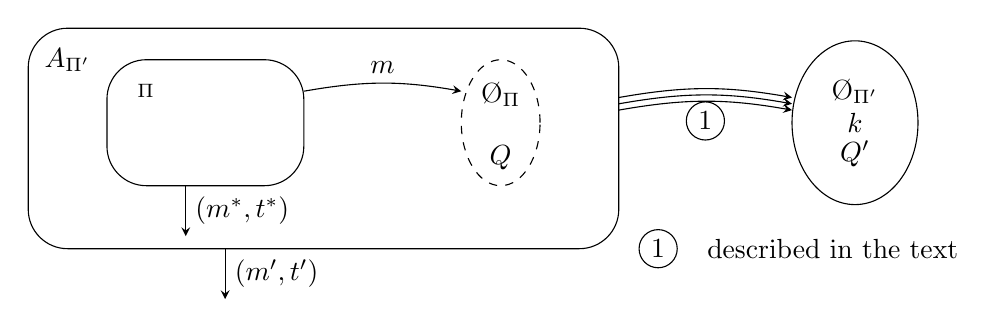
\begin{tikzpicture}[x=1cm, y=0.8cm]
		\draw[rounded corners=0.5cm] (-0.5, 0) rectangle (7, 3.5);
		\draw[rounded corners=0.5cm] (0.5, 1) rectangle (3, 3);
		\draw[dashed] (5.5, 2) ellipse (0.5 and 1);
		\draw (10, 2) ellipse (0.8 and 1.3);
		\draw[-stealth] (3, 2.5) to[bend left=10] node[midway, above] {$m$} (5, 2.5);
		\draw[-stealth]
			(7, 2.4) edge[bend left=10] (9.2, 2.4)
			(7, 2.3) edge[bend left=10] (9.2, 2.3)
			(7, 2.2) to[bend left=10] node[midway, below, draw, circle, inner sep=2pt] {1} (9.2, 2.2)
		;
		\draw[-stealth]
			(1.5, 1) edge node[midway, right] {$(m^*, t^*)$} (1.5, 0.2)
			(2, 0) -- node[midway, right] {$(m', t')$} (2, -0.8)
		;
		\draw
			(1, 2.5) node {$\A_\Pi$}
			(0, 3) node {$A_{\Pi'}$}
			(5.5, 2.1) node[above] {$\O_\Pi$}
			(5.5, 1.8) node[below] {$Q$}
			(10, 2.5) node {$\O_{\Pi'}$}
			(10, 2) node {$k$}
			(10, 1.5) node {$Q'$}
			(7.5, 0) node[draw, circle, inner sep=2pt] {1} ++(0.5, 0) node[right] {described in the text}
		;
		\end{tikzpicture}
		\item $\A'$ should pick a random $r\leftarrow \{0,1\}^{\frac{n}{4}}$, parse m into d blocks $m_1,...,m_d$ and send to its oracle $d$ queries $r\|l\|i\|m_i$ for $i = 1, \ldots, d$.
		After the $d$ queries made to its oracle $O'$, $\A'$ computes $\langle r, t_1, \ldots, t_d \rangle$ where $t_i$ is the answer of the oracle to its $i$th query. He then sends it as an answer to $\A$s query.
		\item For $\Pi$, a forgery is a pair $(m, \langle r, t_1, \ldots, t_d \rangle)$ where $m$ has not been queried before
		and $t_i = \Mac'_k(r\|l\|i\|m_i)$ for $i = 1, \ldots, d$ where $l$ is the length of $m$ and $m = m_1\| \cdots \|m_d$.
		\begin{itemize}
			\item
			If none of its previous query has the same $r$ and $l$, $r\|l\|1\|m_1$ cannot be a query made by $\A'$ and
			$(r\|l\|1\|m_1, t_1)$ is an existential forgery for $\Pi'$ that $\A'$ can output.
			\item
			If 2 previous queries have both $r$ and $l$, then we do not necessarily have an existential forgery.
			However, since $r$ is picked at random ($\A'$ could cheat and make sure that the same $r$ is not picked twice)
			the probability (birthday paradox) of this to happen (if all $m$ have the same $l$ which is the worst case) is approximately
			$\frac{q(n)^2}{2 \cdot 2^n}$ where $q(n)$ is the number of queries made by $\A$.
			\item
			If one unique previous query $m^j$ has this $r$ and $l$, since $m$ is not one of the previous query, there must be $i$
			such that $m_i \neq m_i^j$.
			We know therefore that $r\|l\|j\|m_j$ has never been queried by $\A'$ so $(r\|l\|j\|m_j, t_j)$ is an existential forgery for $\Pi$.
		\end{itemize}
		\item In conclusion, we have
		\begin{align*}
			\Pr[\MacForge_{\A,\Pi}(n) = 1]
			& \leq \Pr[\MacForge_{\A',\Pi'}(n) = 1] + \frac{q(n)}{2^{n+1}}\\
			\epsilon(n)
			& \leq \epsilon'(n) + \frac{q(n)}{2^{n+1}}
		\end{align*}
		so since $\epsilon'(n)$ and $\frac{q(n)}{2^{n+1}}$ are negligible,
		$\epsilon(n)$ is negligible.
	\end{enumerate}

	Alternative answer:
	\begin{enumerate}[start=2]
		\item When $\A_\Pi$ asks for $\Mac_k(m)$, we ($\A_{\Pi'}$) should parse $m=m_1||m_2||\dots||m_d$ with $|m_i|=\frac{n}{4} \, \forall 1\le i \le d=\lceil \frac{l}{n/4}\rceil$ and with the message zero-padded.

		Pick $r \pick \bset^{n/4}$.

		Then, do $d$ requests to $\O_{\Pi'}$ to build $t_i \define \Mac'_k(r||l||i||m_i) \, \forall 1 \le i \le d$.

		Finally, send $t=\langle r, t_1, \dots, t_d\rangle$ to $\A_\Pi$.

		An important question to answer is whether this operation keeps $\A_{\Pi'}$ PPT, with so much requests. To prove this, observe that 1) the message $m$ is generated by a PPT adversary so 2) its length must be polynomial and 3) there is thus at most a polynomial number of blocks and thus 4) we only do a polynomial number of requests to $\O_{\Pi'}$ when $\A_\Pi$ does a request to $\O_\Pi$. So, we are still PPT.

		\item When $\A_\Pi$ outputs $(m^*, t^*)$, we have $t^*=\langle r, t_1, \dots, t_d\rangle$ with $t_i=\Mac'_k(r||l||i|m_i^*)$.

		By hypothesis, there is a chance of $\negl(n)$ that $(m^*, t^*)$ is valid and $m^*$ has never been requested to $\O_\Pi$, i.e., us. Now, we need to extract a valid $(m', t')$ for $\Pi'$. There are three cases:
		\begin{itemize}
			\item If the pair $(r, l)$ has never been used in any of our requests, then $r||l||i||m_i^*$ has never been queried to $\O_{\Pi'}$, and we have our forgery: take any of $(r||l||i||m_i^*, t_i)$.
			\item If $(r, l)$ has been used before, then we need to distinguish between two cases. The first case is if $r$ has been used two or more times before: as $r$ is picked randomly, this event happens with probability $\frac{q(n)}{2^{n/4}}$. In that case, for correct $l$, $\A_\Pi$ could have just rearranged blocks from two previous messages $m^1$ and $m^2$ to build a new message $m^*$. For him, this is an existential forgery against $\Pi$. But for us, all those blocks $r||l||i||m_i^{1, 2}$ have been queried to our oracle before, and so none of them are fresh, and this is not a forgery against $\Pi'$.
			\item If $(r, l)$ has been used before and $r$ has only been used once, then there is a past message $m^1$ whose tag used this $r$. Let's compare the two messages:
			\begin{align*}
			m^1 &\rightarrow m_1^1||m_2^1||\dots||m_d^1 \rightarrow \langle r, \Mac'_k(r||l||1||m_1^1), \dots\rangle \\
			m^* &\rightarrow m_1^*||m_2^*||\dots||m_d^* \rightarrow \langle r, \Mac'_k(r||l||1||m_1^*), \dots\rangle
			\end{align*}
			As $m^*$ is a forgery against $\Pi$, $m^1 \neq m^*$, so $\exists j \suchthat m_j^1 \neq m_j^*$. For this $i$, the corresponding $(r||l||j||m_j^*, t_j)$ is a forgery against $\Pi'$.
		\end{itemize}
		If now we compute it,
		\begin{align*}
		\negl'(n) = \Pr[\MacForge_{\A_{\Pi'},\Pi'}(n)=1] &\ge \Pr[\MacForge_{\A_\Pi,\Pi}(n)=1 \\
		&\quad \wedge \text{ We can build a forgery from it}] \\
		&\ge \Pr[\MacForge_{\A_\Pi,\Pi}(n)=1] \cdot \left(1-\frac{q(n)}{2^{n/4}}\right) \\
		&= \negl(n) \left(1-\frac{q(n)}{2^{n/4}}\right)
		\end{align*}
		As we know that $\Pi'$ is EUF-CMA, then $\negl'(n)$ must be negligible, so the whole right-hand side must be negligible too, and so $\negl(n)$ must be negligible.

		Other said, if $\negl(n)$ is non-negligible, then the right-hand side is non-negligible (the term in parenthesis is negligibly close to $1$), and so $\negl'(n)$ must be non-negligible too.
	\end{enumerate}
\end{solution}



\subsection{Exercise 3 (Authenticated encryption and sPRP)}

\copypaste{4}{2}



\subsection{Exercise 4 (Authenticated encryption)}

Let $\Pi=(\Gen, \Enc, \Dec)$ be an authenticated encryption scheme where $0\not\in \C$ (that is, the string ``0'' is not a possible ciphertext for $\Pi$). Consider the following scheme $\Pi' \define (\Gen', \Enc', \Dec')$ with:
\begin{itemize}
	\item $\Gen'=\Gen$
	\item $\Enc'=\Enc$
	\item $\forall k: \Dec'(c) = \begin{cases} \Dec(c) \text{ if } c\neq 0, \\ 0 \text{ if } c=0. \end{cases}$
\end{itemize}
\begin{enumerate}
	\item Is $\Pi'$ unforgeable?
	\item Is $\Pi'$ CCA secure?
\end{enumerate}


\begin{solution}
	\begin{enumerate}
		\item It is not unforgeable. To see this, simply build the following adversary $\A$:
		\begin{enumerate}[label=(\arabic*)]
			\item The oracle-challenger chooses $k \pick \K$.
			\item We have no query to do to the oracle.
			\item Output $c=0$.
		\end{enumerate}
		By definition, $\Dec'_k(0)=0 \, \forall k$, so it is a valid message. So $\Pr[\EncForge_{\A, \Pi'}(n)=1]=1$.
		\item It is CCA-secure (sure at 95\%). To show this, let's do a reduction. If we have a PPT adversary $\A_{\Pi'}$ against $\Pi'$, we can build an adversary $\A_\Pi$ against $\Pi$ and run the following experiment (from the viewpoint of $\A_\Pi$):
		\begin{enumerate}[label=(\arabic*)]
			\item The oracle-challenger chooses $k \pick \K$.

			\item First query phase:
			\begin{itemize}
				\item When $\A_{\Pi'}$ asks for $\Enc'_k(m)$ of a message $m$, we simply forward the request to $\O_\Pi$, receive $c=\Enc_k(m)$, and return it to $\A_{\Pi'}$
				\item When $\A_{\Pi'}$ asks for $\Dec'_k(c)$ of a ciphertext $c$, if $c=0$, then we return $0$, and if $c\neq 0$, we forward the request to $\O_\Pi$, receive $m=\Dec_k(c)$ and return it to $\A_{\Pi'}$.
			\end{itemize}

			\item $\A_{\Pi'}$ outputs its messages $m_0, m_1$. We output them.

			\item The challenger-oracle picks $b\pick \bset$, returns $c^*=\Enc_k(m_b)$, sends that to us, and we forward it to $\A_{\Pi'}$.

			\item Second query phase, similar to the first one, with the exception that $\A_{\Pi'}$ cannot ask for $\Dec'_k(c^*)$.

			\item $\A_{\Pi'}$ outputs its guess $b'$, and we output $b''=b'$.
		\end{enumerate}
		The adversary $\A_{\Pi'}$ is exactly in the correct conditions, our adversary $\A_\Pi$ is PPT, and we output the same value, so $\Pr[\PrivKcca[\A_\Pi, \Pi](n)=1]=\Pr[\PrivKcca[\A_{\Pi'}, \Pi'](n)=1]=\Pr[b'=b]=\Pr[b''=b]=\negl$
		and, as we know that $\Pi$ is CCA-secure, then we have that $\Pi'$ is CCA-secure. This ``zero-filling'' has no impact on the CCA-security, only on the unforgeability.
	\end{enumerate}
\end{solution}



\subsection{Exercise 5}
% This practical session was entirely corrected by the teaching assistants so, there is no need to correct the solutions.

Let $F$ be a PRF. Below, we describe three \textit{insecure} \emph{variable-length} message authentication codes (\textit{a.k.a.} MACs), $\Pi_1$, $\Pi_2$ and $\Pi_3$, which all use the same key generation algorithm $\G$. The message space is \emph{any (non negative) number} of message blocks in $\{0,1\}^n$, where $n$ is the security parameter.
%
\begin{description}
	\item[$\G(1^n)$] outputs a random key $k\gets\bset^n$.
\end{description}
%
The scheme $\Pi_3$ is built from $\Pi_2$ which is itself built from $\Pi_1$ as an (unsuccessful) attempt to ``patch'' the previous scheme:
%
\begin{description}
	\item[$\Pi_1=(\Gen,\Mac^1,\Vrfy^1)$:]
	\emph{``Deterministic MAC -- Chaining PRFs''}

	$\Mac^1_k(m_1,\ldots,m_\ell)$ computes $t_1=F_k(m_1)$ as well as
	$t_i=F_k(m_i\oplus t_{i-1})$, for $i=2$ to $\ell$, and returns $t \define t_\ell$ (note that only the last block is returned).

	$\Vrfy^1_k((m_1,\ldots,m_{\ell}),t)$ outputs $1$ if
	$\Mac^1_k(m_1,\ldots,m_{\ell})=t$, and 0 otherwise.
	\item[$\Pi_2=(\Gen,\Mac^2,\Vrfy^2)$:]
	\emph{``Padding a random message block in the end''}

	$\Mac^2_k(m_1,\ldots,m_\ell)$ first picks a random $r\gets\{0,1\}^n$ and
	then runs $t=\Mac_k^1(m_1,\ldots,m_\ell,r)$ and outputs $(r,t)$.

	$\Vrfy^2_k((m_1,\ldots,m_{\ell}),(r,t))$ outputs $1$ if
	$\Mac^1_k(m_1,\ldots,m_{\ell},r)=t$, and 0 otherwise.

	\item[$\Pi_3=(\Gen,\Mac^3,\Vrfy^3)$:]
	\emph{``Padding a random message block in the beginning''}

	$\Mac^3_k(m_1,\ldots,m_\ell)$ first picks a random $s\gets\{0,1\}^n$ and
	then runs $(r,t)=\Mac_k^2(s,m_1,\ldots,m_\ell)$ and outputs $(r,s,t)$.

	$\Vrfy^3_k((m_1,\ldots,m_{\ell}),(r,s,t))$ outputs $1$ if
	$\Mac^1_k(s,m_1,\ldots,m_{\ell},r)=t$, and 0 otherwise.
\end{description}

\begin{enumerate}
	\item Describe $\Mac_k^3(m_1,\ldots,m_\ell)$ explicitly in term of computations
	of $F_k$ (and $\oplus$ of course).
	\item Show the correctness of $\Pi_3$.
	\item Mount a forgery attack on these MACs.
\end{enumerate}

\begin{solution}
	\begin{enumerate}
		\item For random $r,s\leftarrow \{0,1\}^n$,
		$\Mac^3_k(m_1,\ldots,m_\ell)$ computes $t_0=F_k(s)$, then $t_i=F_k(m_i \oplus t_{i-1})$ for $i=1$ to $\ell$, and finally
		$t_{\ell+1}=F_k(r\oplus t_\ell)$.
		It outputs $(r,s,t)$ where $t \define t_{\ell+1}$.

		\item Using the description of $\Mac^1_k$, on inputs $(s,m_1,\ldots,m_\ell,r)$ it gives $t'_1=F_k(s)$, for $i=1$ to $\ell$, $t'_{i+1}=F_k(m_i \oplus t'_i)$, and $t'_{\ell+2}=F_k(r \oplus t'_{\ell+1})$. $t'_{\ell+2}$ is the output, or equivalently:
		\begin{align*}
		F_k(r \oplus t'_{\ell+1}) &= F_k \bigg(r \oplus F_k \Big(m_\ell \oplus F_k \big( m_{\ell-1} \oplus \dots F_k(m_1\oplus F_k(s)) \dots \big)\Big)\bigg)\\
		&=t.
		\end{align*}

		\item These MACs are not even one-time secure:
		\begin{description}
			\item $\Pi_1$: (1) query $\Mac^1_k(m)$ on any $m\in\bset^n$ and get the tag $t=F_k(m)$;

			(2) output $((m,m\oplus t),t)$.

			$t_1=F_k(m)$, $t_2=F_k(m\oplus t \oplus t_1)= F_k(m \oplus 0)=t$.

			\item $\Pi_2$: (1) query $\Mac^2_k(m)$ on any $m\in\{0,1\}^n$ and get the tag $(r,t)$, where $t=F_k(F_k(m)\oplus r)$;

			(2) output $((m,r,m\oplus t),(r,t))$.

			$t_1=F_k(m)$, $t_2=F_k(F_k(m)\oplus r)=t$, $t_3=F_k(t\oplus m \oplus t)=F_k(m)$, $t_4=F_k(F_k(m)\oplus r)=t$.

			\item $\Pi_3$: (1) query $\Mac^3_k(m)$ on any $m\in\{0,1\}^n$ and get the tag $(r,s,t)$, where $t=F_k( F_k(F_k(s) \oplus m)  \oplus r)$

			(2) output $((m,r,s\oplus t,m),(r,s,t))$.

			$t_1=F_k(s)$, $t_2=F_k(F_k(s) \oplus m)$, $t_3=F_k(F_k(F_k(s) \oplus m) \oplus r)=t$, $t_4=F_k(t \oplus s \oplus t)= F_k(s)$, $t_5=F_k(F_k(s)\oplus m)$, $t_6=F_k( F_k(F_k(s) \oplus m)  \oplus r)=t$.
		\end{description}
	\end{enumerate}
\end{solution}



\subsection{Exercise 6}
% This practical session was entirely corrected by the teaching assistants so, there is no need to correct the solutions.

Let $F$ be a pseudorandom function, $G$ be a pseudorandom permutation, $T$ be a public $n$-bit constant, $k$ be a $n$-bit secret key, $m$ be a $n$-bit message, $IV$ be a $n$-bit random value chosen by the party computing the encryption (resp.~MAC) before each operation. Among the following constructions, determine the ones that would be acceptable and justify your answer. (Your justifications can rely on results that have been presented during the class.)

\begin{enumerate}
	\item $\Enc_k(m) \define F_k(m \oplus T)$ as an encryption scheme secure against
	eavesdropping.

	\item $\Enc_k(m) \define G_k(m \oplus T)$ as an encryption scheme secure against eavesdropping.

	\item $\Enc_k(m) \define G_k(m \oplus T)$ as an encryption scheme secure against a CPA-adversary.

	\item $\Enc_k(m) \define (IV,G_k(m \oplus T \oplus IV))$ as an encryption scheme secure against a CPA-adversary.

	\item $\Mac_k(m) \define F_k(m \oplus T)$ as a MAC scheme existentially unforgeable under an
	adaptive chosen-message attack.

	\item $\Mac_k(m) \define (IV,G_k(m\oplus IV \oplus T))$ as a MAC scheme
	existentially unforgeable under an adaptive chosen-message attack.
\end{enumerate}


\begin{solution}
	\begin{enumerate}
		\item No, decryption does not work in general, as we do not
		necessarily know how to invert a PRF.

		\item 	Yes, it is secure.  The reduction to the PRP security can work as follows:
		the reduction gets $m_0$ and $m_1$ from the eavesdropper
		adversary, picks a random bit $b$, sends $m_b \oplus T$ to the
		challenger and receives a value $c$ that it sends back to the eavesdropper
		adversary. This adversary has a probability exactly $1/2$ to
		guess $b$ if $c$ comes from a random permutation, and a
		probability $1/2 + \negl$ to guess $b$ if $c$ comes from a
		pseudorandom permutation. The reduction can therefore claim that
		it sees a PRP every time the adversary makes a successful
		guess. The difference between the two probabilities is $\negl$.
		So, if $F$ is a PRP, $\epsilon$ must be negligible.

		\item 	No: it is not probabilistic. CPA security is not achievable with deterministic encryption.

		\item We first observe that the $\oplus T$ does not matter:
		since $T$ is public, the adversary has the possibility to adapt
		its choice of $m$ in order to cancel it.  Now, if we abstract
		from $T$, this is exactly the CBC encryption mode, which we know
		to be CPA-secure.

		\item Again, we observe that the $\oplus T$ does not matter: since
		$T$ is public, the adversary has the possibility to choose exactly
		on which value $F_k$ will be applied. Now, if we abstract from $T$,
		this is exactly the basic MAC scheme from the class, which is secure.

		\item This is insecure. Given one tag $(IV, t)$ on a message
		$m$, the adversary can produce a valid tag $(IV', t)$ on the
		message $m' = m \oplus IV \oplus IV'$ for any $IV'$.
	\end{enumerate}
\end{solution}



\subsection{Exercise 7 (Blue-ray security)}

The movie industry wants to protect digital content distributed on DVD's. We study
one possible approach. Suppose there are at most a total of $n$ DVD players in the world (e.g.
$n=2^{32}$). We view these n players as the leaves of a binary tree of height $\log_2 n$.
Each node $\nu_j$ in this binary tree contains an AES key $K_j$ such that
$\mathrm{Enc}_{K_j}:\{0,1\}^l\rightarrow\{0,1\}^l$ is assumed to be a \emph{secure} encryption.
These keys are kept secret from consumers and are fixed for all time.
At manufacturing time each DVD player is assigned a serial number $i\in\left[0,n-1\right]$.
Consider the set $S_i$ of $\log_2(n+1)$ nodes along the path from the root to leaf number
$i$ in the binary tree. The manufacturer of the DVD player embeds in player number $i$ the
$\log_2(n+1)$ keys associated with the nodes in $S_i$. In this way each DVD player ships with
$\log_2(n+1)$ keys embedded in it (these keys are supposedly inaccessible to consumers).

\begin{enumerate}
	\item Since all DVD players have the key \emph{root} (noted $K_{root}$),
	      find a way to protect the content $M\in\{0,1\}^l$ of a DVD such that all players can decrypt
	      the movie (and then read it).
	\item Now suppose that a hacker has been able to extract the key $K_{root}$ embedded in his
	      DVD player and has published it on the Internet.
	      Show how the movie industry can encrypt the contents of a new DVD $M\in\{0,1\}^l$ such that only
	      the owners of a DVD player can read it.
	      Note that the movie indutry does not want to produce several encryptions of the
	      same content $M$ \emph{i.e.} there will be a single manner to protect the DVD.
	\item Suppose the $\log_2n$ keys embedded in DVD player number $r$ are exposed by hackers
	      and published on the Internet. Show that when the movie industry is about to
	      distribute a new DVD movie they can encrypt the contents of the DVD using a
	      ciphertext of size $l\!\cdot\!(1+\log_2n)$ so that all DVD players can decrypt the movie except
	      for player number $r$. In effect, the movie industry disables player number $r$.

	      \emph{Hint: the DVD will contain $\log_2n$ ciphertexts where each ciphertext is the
	      encryption of a unique K under certain $\log_2n$ keys from the binary tree.}
\end{enumerate}


\begin{solution}
  \begin{enumerate}
    \item Encrypt all the DVDs with $K_\text{root}$, i.e. build the ciphertext: $c_{root}=Enc_{K_{root}}(M)$
    \item At the beginning of the DVD, encrypt a random key $K$ twice (using $K_2$ and then $K_3$): $Enc_{K_2}(K)$ and $Enc_{K_3}(K)$.

      We then encrypt all the content $M$ of the DVD using $K$. (We suppose $K_1$ is $K_{\text{root}}$)
      $K_2$ and $K_3$ are the keys associated to the 2 childs of the root.

      \textbf{Other possibility}

      Simply encrypt the contents of the new DVD M as: $Enc_{K2}(M)||Enc_{K3}(M)$. This way, each DVD player is still able to decrypt the content, but nobody that only has $K_{root}$.
    \item
      For every node $i$ on the path from the root to $r$, we must add an encryption of $K$ with the key of its child that is not in the path.
      For example, if $r = 10$ and $n = 16$, we must include the bold keys,
      so we will include the encryption of $K_7$ in a DVD which is quite something.

      \textbf{Expressed differently}

      If we want to disable the DVD player 11 for example, we can create a new ciphertext as: $c_{disable} = Enc_{K_2}(M)||Enc_{K_7}(M)||Enc_{K_{12}}(M)||Enc_{K_{player10}}(M)$

      \begin{center}
        \Tree [.{$K_{\text{root}} = K_1$}
          [.{$\mathbf{K_2}$}
            [.{$K_4$}
              [.{$K_8$}
                [.{0} ]
                [.{1} ]
              ]
              [.{$K_9$}
                [.{2} ]
                [.{3} ]
              ]
            ]
            [.{$K_5$}
              [.{$K_{10}$}
                [.{4} ]
                [.{5} ]
              ]
              [.{$K_{11}$}
                [.{6} ]
                [.{7} ]
              ]
            ]
          ]
          [.{$K_3$}
            [.{$K_6$}
              [.{$\mathbf{K_{12}}$}
                [.{8} ]
                [.{9} ]
              ]
              [.{$K_{13}$}
                [.{\textbf{10}} ]
                [.{11} ]
              ]
            ]
            [.{$\mathbf{K_7}$}
              [.{$K_{14}$}
                [.{12} ]
                [.{13} ]
              ]
              [.{$K_{15}$}
                [.{14} ]
                [.{15} ]
              ]
            ]
          ]
        ]
      \end{center}
  \end{enumerate}
\end{solution}



\subsection{Exercise 8 (Authenticated encryption, or not)}

\copypaste{10}{1}



\subsection{Exercise 9 (Authenticated encryption)}

\copypaste{4}{1}



% TODO
\subsection{Exercise X (Mode of operation)}
Show formally that ECB-mode encryption does not have indistinguishable encryptions in the presence of an eavesdropper.
\begin{solution}
  Let say we have to split the message into $m$ messages of $n$ bits.
  Choosing $m_0 = M_0 \| M_0 \| \cdots \| M_0$ and $m_1 = M_1 \| M_2 \| \cdots \| M_m$ with $M_i \neq M_j$ for $i \neq j$,
  if $b = 0$, $\A$ will get $c = C_0 \| C_0 \| \cdots \| C_0$ for some $C_0 \in \C$. But if b=1, $\A$ will get $c = C_1 \| C_2 \| \cdots \| C_m$ for some $C_i \in \C$.

  An adversary $\A$ can output $b = 0$ iff all the $C_i$s are equals.
  We have
  \[ \Pr[\PrivK^{\text{eav}}_{\A,\text{ECB}}(nm)] = \frac{1}{2} + \frac{1}{2} = 1 \]
  since the $C_i$ cannot be equal if $b = 1$ since we use a PRP.
  If two different $M_i$ were encrypted as same $C_i$, decryption wouldn't be possible.
\end{solution}
